\begin{figure}
\centering
\fbox{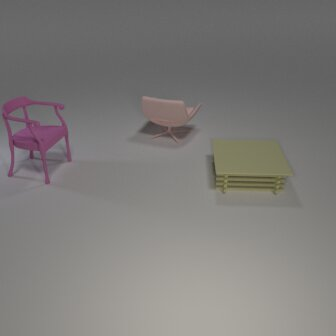
\includegraphics[width=0.4\linewidth]{figures/samples/scene_level_6dof.jpg}}
\begin{minted}[breaklines]{python}
add(rotation=(0.999, 0.024, -0.042, 0.024, 0.496, 0.868), color='Olive Green', loc=(2.228, 0.057, -10.362), shape='tables_0010')
add(rotation=(0.934, 0.177, -0.310, 0.163, 0.561, 0.812), loc=(0.032, 1.816, -12.639), color='Melon', shape='chairs_0055')
add(loc=(-3.707, 1.009, -10.332), rotation=(-0.235, 0.481, -0.845, -0.689, -0.696, -0.204), shape='chairs_0008', color='Red Violet')
\end{minted}
\caption{\textbf{ShapeNet 6-DoF Train Sample.} (\cref{sssec:scene_6dof})}
\label{fig:code_scene_6dof}
\end{figure}